\section{Scope}\label{sec:scope}

This thesis will work in a server-relay-client environment.
A relay is a special type of server with individual 
connections to the previous and the next hop in the network path.
In our case the previous and next hop will already be the media server and 
the client, respectively.
This is visualized in~\autoref{fig:relay-setup}.
\vspace{0.5cm}
\begin{figure}[H]
    \centering
    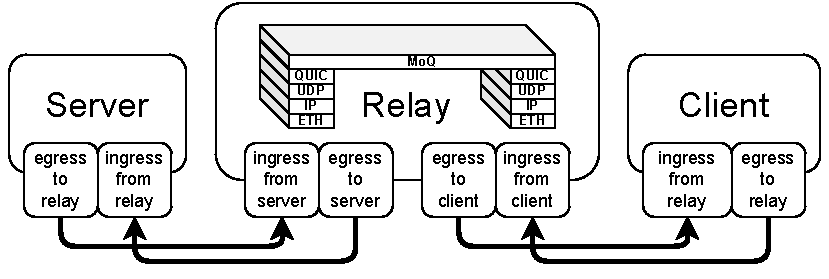
\includegraphics[width=0.8\textwidth]{figures/02_background/general-relay.drawio.pdf}
    \caption[Server-Relay-Client-Setup]{Relay setup.}\label{fig:relay-setup}
\end{figure}
The task of a relay is to pass on the traffic it receives from its predecessor
to one or more successors.
To achieve this, a packet goes all the way up the relay's application layer.
We aim to avoid such an expensive traversal up the network stack.

The main improvement this thesis aims to achieve is shortening a packet's critical path from a media server to a client.
This will be done by avoiding the immediate need for a packet traversal up the network stack to the application layer.
Instead, any communication with the application layer will happen in a delayed fashion (after the packet is sent) by utilizing 
eBPF maps for storing any necessary (meta-)~information.
This communication between userspace and the eBPF program is required because relays in MoQ are an application layer concept.
That means the QUIC connections from the relay to the server and from the relay to the client will be different, and the packets that have been eBPF-forwarded to egress directly will need changes in their header data to match the state of the outgoing client connection.  

This approach is highly dependent on the used standards and protocols.
This thesis will operate on top of the QUIC protocol~\parencite{rfc-9000} and the MoQ
transport protocol~\parencite{draft-moqtransport}.
For the application layer, the quic-go library~\parencite{quic-go-repo} will provide the implementation and 
any additional (non-eBPF) program will also be written in Go.
Since the setup is dependent on retrieving data from eBPF maps, the QUIC library providing the RFC implementation 
will need some adaptations.
We will mainly introduce simple function pointer style additions that allow the adapted library to be run 
both with and without the eBPF setup.
The developer of the relay will then also have more freedom to set up the eBPF part of the relay as they see fit
since the Go code that will interact with eBPF parts will also have to be provided by said developer.

Additionally, we will run a performance analysis on our relay implementation to confirm this approach's potential.
These performance tests will look at the raw delay speedup and the impact on CPU utilization this setup has.
All the tests will be done in a lab-like environment to isolate the performance changes as best as possible
from any outside noise.
Most payloads used will only contain dummy data since our approach does not interfere with payload contents 
and there is no need for creating and using actual media stream data.

Despite our approach only considering QUIC and MoQ, we will argue that the general idea of our setup will be independent of
any of these protocols and can be changed to fit one's needs.

With this, we will provide answers to the research questions regarding packet-redirection, communication between userspace and eBPF
as well as setup-generalization.
Regarding the question of how to handle the encryption of the packets, we will not focus on this, since we did not find a suitable hardware offload that would have allowed for en- and decryption after and before the used eBPF hook points, respectively.
Instead, we will emulate this behavior by turning off the encryption in the QUIC library itself, which will provide a similar result.

% TODO: better spot for this part?
% The only two assumptions that were made are that it is possible for the protocol to store meta-information like a 
% packet-priority in the packet itself and that our relay has access header data even if it is part of encrypted areas.
% For the former point, we utilized one byte of the QUIC Connection-Id as a proof of concept, but in later implementations 
% this could be changed to using any separately defined application header that allows storing such 
% information.
% Since we assume full knowledge over the eBPF setup when the payload is created at the server (because server and 
% relay are generally both part of the same CDN), this assumption is not a big stretch.
% The latter point can be achieved by having a hardware offload of en- and decryption onto a smartNIC\@.
% Since such an offload was not yet available to us, we turned off en- and decryption directly within the 
% QUIC library itself, which provides a similar result.
